\documentclass[tikz, border=0px]{standalone}
\usepackage{tikz}
\usetikzlibrary{shapes,arrows}

\tikzstyle{startstop} = [rectangle,rounded corners,minimum width=3cm,minimum height=1cm,align=center,draw=black, text width=2.5cm, fill=green!30]

\tikzstyle{therapy} = [trapezium, trapezium left angle =70, trapezium right angle=110, minimum width=2cm, minimum height = 1cm, centered,draw=black,align=center, text width=2cm, fill=orange!30]

\tikzstyle{decision} = [diamond, minimum width = 3cm, minimum height = 3cm, text centered, draw=black, text width = 2cm,align=center,fill=blue!30]

\tikzstyle{arrow} = [thick, ->, >=stealth]
\tikzstyle{doublearrow} = [<->, thick, >=stealth]

\begin{document}
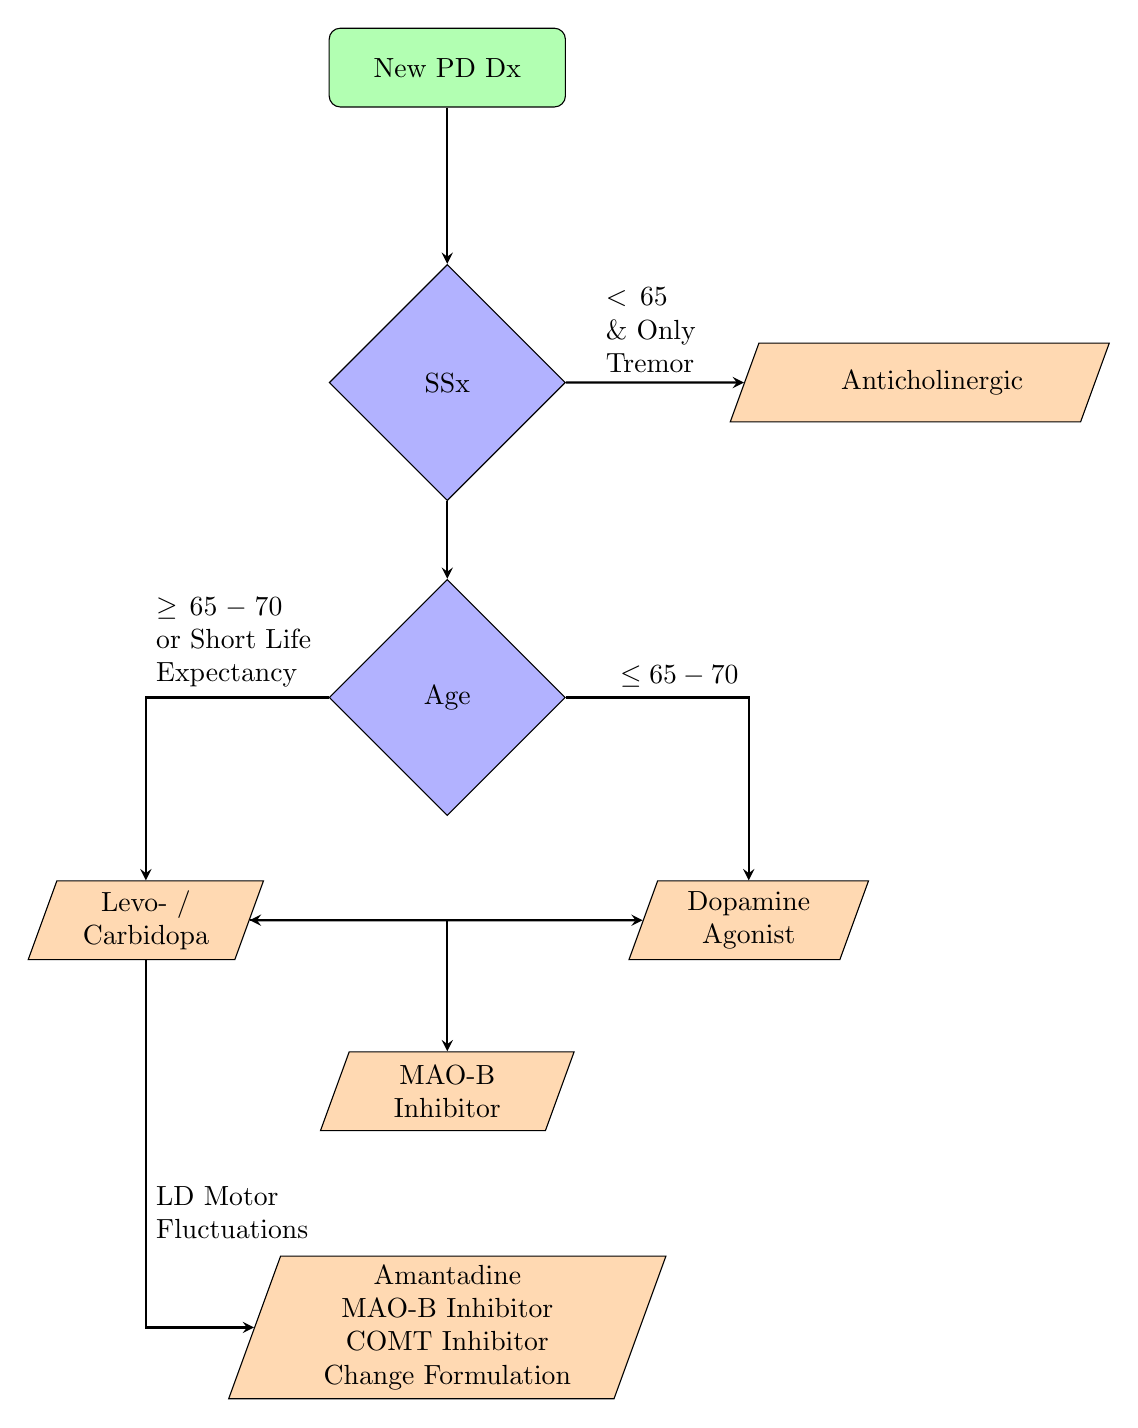
\begin{tikzpicture}[node distance=4cm]

\node (start) [startstop] {New PD Dx};
\node (justTremor) [decision, below of=start] {SSx};
\node (age) [decision, below of=justTremor] {Age};
\node (da) [therapy, below right of=age, xshift=1cm] {Dopamine Agonist};
\node(ldopa) [therapy, below left of=age, xshift=-1cm] {Levo- / Carbidopa};
\node (antichol) [therapy, right of=justTremor, xshift=2cm] {Anticholinergic};
\node (maob) [therapy, below of=age, yshift=-1cm] {MAO-B Inhibitor};
\node (addOns) [therapy, below of=maob, text width=4cm, yshift=1cm] {Amantadine\\ MAO-B Inhibitor\\ COMT Inhibitor\\ Change Formulation};

\draw [arrow] (start) -- (justTremor) ;
\draw [arrow] (justTremor) -- node [anchor=south, text width=1.25cm] {$<65$ \& Only Tremor} (antichol);
\draw [arrow] (justTremor) -- (age);
\draw [arrow] (age) -| node [anchor=south west, text width = 2cm] {$\ge 65-70$ or Short Life Expectancy} (ldopa);
\draw [arrow] (age) -| node [anchor=south east] {$\le 65-70$} (da);
\draw [doublearrow] (ldopa) -- (da);
\draw [arrow] (ldopa) -| (maob);
\draw [arrow] (ldopa) |- node [anchor=south west, yshift=1cm, text width=2cm] {LD Motor Fluctuations} (addOns);

\end{tikzpicture}
\end{document}